\documentclass[a4paper,10pt]{article}
\usepackage[french]{babel}
\usepackage[margin=.8in]{geometry}
\usepackage[T1]{fontenc}
\usepackage[utf8]{inputenc}
\usepackage{graphicx}
\usepackage{float}
\usepackage{tabularx}
\usepackage{array}
\usepackage{hyperref}
\hypersetup{urlbordercolor={1 .5 0}}
\usepackage{newcent}
\selectfont
\usepackage{framed}
\setlength{\parindent}{0pt}
\begin{document}
\pagenumbering{gobble}

{\Large John \sc Gliksberg}
\hrulefill\\[-.47cm]
\begin{minipage}{0.8\textwidth}
\begin{flushleft}
\vspace{.5cm}
%29 ans, né le 25 juin 1994\\
21 bis rue Jean Leclaire, 75017 Paris\\[.2cm]
+33 6 40 60 76 95\\
\href{mailto:jg.trosh@gmail.com}
{jg.trosh@gmail.com}\\[.2cm]
Langues maternelles français \& anglais\\
Permis B, véhicule personnel
\end{flushleft}
\end{minipage}%
\begin{minipage}{0.2\textwidth}
\begin{figure}[H]
\begin{flushright}
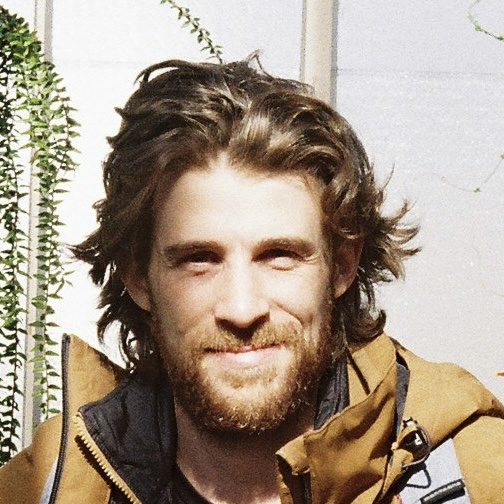
\includegraphics[height=3cm]{johnpic}
\end{flushright}
\end{figure}
\end{minipage}\\

\begin{center}
    \framebox{
        \parbox{335\unitlength}{
            \centering\large\sc
	    Jeune docteur \\
            Ingénieur recherche spécialisé HPC
        }
    }
\end{center}
\vspace{.3cm}

%{\large\bf Profil}
%\hrulefill\\[.3cm]
%{\setlength{\extrarowheight}{.2cm}
%Je suis très motivé, adaptable et ai développé une approche responsable
%dans toutes les tâches que j'entreprends.
%Mes managers et superviseurs apprécient la fiabilité de mes analyses
%et ma capacité de compréhension et de résolution de problèmes techniques.
%Je suis avide de découvertes, autant prêt à travailler en équipe que
%de mon initiative, en français autant qu'en anglais.
%}
%\vspace{.3cm}

{\large\bf Études}
\hrulefill\\[.3cm]
{\setlength{\extrarowheight}{.2cm}
\begin{tabularx}{\textwidth}{lX}
2017\---2022 &
{\bf Thèse CIFRE} en cotutelle internationale
\newline
Université de Versailles Saint-Quentin-en-Yvelines (UVSQ), \newline
Universidad de Castilla-La-Mancha (UCLM), \newline
Atos \newline
\og \href{https://theses.hal.science/tel-03992998}{Nouveaux algorithmes de routage pour supercalculateurs hétérogènes exaflopiques} \fg \newline
1 publication en journal, 2 en conférences, 1 en workshop \\
2015\---2016 &
\href{https://chps.uvsq.fr}
{\bf Master Informatique Haute Performance \& Simulation}
\newline
UVSQ \\
2014 &
\href{https://www.uvsq.fr/double-licence-mathematiques-et-physique-343617.kjsp}
{\bf Double Licence Mathématiques \& Physiques}
\newline
UVSQ \\
2011 &
\href{https://www.education.gouv.fr/cid20999/l-option-internationale-du-baccalaureat-o.i.b.html}
{\bf Baccalauréat Scientifique OIB} (option internationale)
\newline
Lycée de Sèvres (SIS) \\
2010 &
\href{https://www.cambridgeenglish.org/exams/proficiency/}
{\bf Certificate of Proficiency in English} (CPE)
\---- {\bf Anglais niveau C2}
\newline
University of Cambridge
\end{tabularx}}
\vspace{.3cm}

%{\large\bf Portfolio}
%\hrulefill\\[.2cm]
%Langages : C, C++, Python 2/3, Lua, Go, Scilab, Matlab, Fortran, Cuda \\
%Librairies : Blas, Lapack, Vtk, MPI, OpenMP \\
%Outils : Linux, bash/zsh, vim/emacs, Paraview, Makefile, \LaTeX, git/svn \\
%Misc : html/css, js, php, sql
%\vspace{.3cm}

{\large\bf Activités professionnelles}
\hrulefill\\[.2cm]
{\setlength{\extrarowheight}{.2cm}
\begin{tabularx}{\textwidth}{lX}
2016\--- &
{\bf Atos Big Data \& Security (ex-Bull)}, Bruyères-le-Châtel
\newline
Ingénieur recherche \---- logiciel management réseau HPC BXI, expert routage \newline
Développement en C et Python, travail en équipe Agile, expertise Git \newline
Membre d'un projet de travail en collaboration européenne \newline
2 dépots de brevets, 2 CIR \\
2016 &
\href{https://3ds.com}{\bf Dassault Systèmes}, Vélizy-Villacoublay \newline
Stage de 6 mois à temps complet \---- chercheur logiciel \newline
Simulation de solides déformables avec réduction d'ordre de modèle, portage GPU \\
2015 &
\href{https://www.scilab.com}{\bf Scilab-Enterprises}, Versailles
\newline
Stage de 4 mois à temps complet \---- développeur logiciel open-source
\newline
Industrialisation de modules Scilab, développements sur Scilab 6
\\
2014 &
Laboratoire de physique
\href{https://www.gemac.uvsq.fr/}
{\bf GEMaC\--CNRS\--UVSQ}, Versailles
\newline
Stage de 4 mois à temps partiel
\newline
\og Étude visuelle de transitions de phase dans des monocristaux\fg
\\
2013\---2015 &
Tuteur et formateur en anglais,
\href{https://www.cerel.uvsq.fr/}
{\bf CEREL \makeatletter @ \makeatother UVSQ} \newline
Tutorats en groupes \----
Cours individuels pour étudiants malentendants
\end{tabularx}}
\vspace{.3cm}

{\large\bf Autres activités}
\hrulefill\\[.3cm]
{\setlength{\extrarowheight}{.15cm}
\begin{tabularx}{\textwidth}{lX}
2023\---2024 &
\href{https://travelbellies.blog}{Tour du monde} pendant 11 mois (congé sabbatique) \\
2014\---2015 &
Coordinateur et co-fondateur de l'association
\href{https://www.facebook.com/pages/Seventy-Eighters/508772502567015}
{Seventy-Eighters}
\makeatletter @ \makeatother UVSQ \\
2013\---2015 &
Élu étudiant au Conseil UFR
\makeatletter @ \makeatother UVSQ
\end{tabularx}}
%\newline
%{\setlength{\extrarowheight}{.15cm}
%\begin{tabularx}{\textwidth}{X}
%Dessin (portraits, bande-dessinée) \hfill
%Lecture, cinéma (SF) \hfill
%Tennis de table \\
%Musique (électronique, bossa nova, jazz) \hfill
%Projet Euler \hfill
%Animation procédurale
%\end{tabularx}}

%\newpage
%
%{\Large John Gliksberg}
%\hrulefill\\
%\newline
%Aged 21, born 25 June 1994\\
%14 rue Anatole France, 92310 Sèvres, France\\[.1cm]
%+33 6 40 60 76 95\\
%\href{mailto:jg.trosh@gmail.com}
%{jg.trosh\makeatletter @\makeatother gmail.com}\\[.1cm]
%Native speaker in French \& English\\
%Driving licence and vehicle
%
%\begin{center}
%    \framebox{
%        \parbox{379\unitlength}{\centering\large\sc
%            Seeking a challenging 6-month end-of-studies internship \\
%            MSc High Performance Computing \& Simulation
%        }
%    }
%\end{center}
%\vspace{.3cm}
%
%{\large\bf Profile}
%\hrulefill\\[.3cm]
%{\setlength{\extrarowheight}{.2cm}
%I am a highly motivated and adaptable person and have developed
%a mature and responsible approach to any task I undertake.
%My managers and supervisors appreciate my solid analytical skills
%and ability to understand and solve problems.
%I am eager to learn and am equally at ease working in a team
%or on my own initiative, in French or in English.
%}
%\vspace{.3cm}
%
%{\large\bf Education}
%\hrulefill\\[.3cm]
%{\setlength{\extrarowheight}{.2cm}
%\begin{tabularx}{\textwidth}{lX}
%2015 \---- 2016 &
%\href{https://mihps.prism.uvsq.fr}
%{\bf M.Sc. (2nd year), High Performance Computing \& Simulation}
%\newline
%Université de Versailles Saint-Quentin-en-Yvelines (UVSQ) \\
%2015 &
%\href{https://mihps.prism.uvsq.fr}
%{\bf M.Sc. (1st year), High Performance Computing \& Simulation}
%(bien, major)
%\newline
%Université de Versailles Saint-Quentin-en-Yvelines (UVSQ) \\
%2014 &
%\href{https://www.uvsq.fr/double-licence-mathematiques-et-physique-343617.kjsp}
%{\bf B.Sc., Mathematics \& Physics}
%\newline
%Université de Versailles Saint-Quentin-en-Yvelines (UVSQ) \\
%2011 &
%\href{https://www.education.gouv.fr/cid20999/l-option-internationale-du-baccalaureat-o.i.b.html}
%{\bf Scientific Baccalaureate OIB} (international option)
%\newline
%Lycée de Sèvres (SIS) \\
%2010 &
%\href{https://www.cambridgeenglish.org/exams/proficiency/}
%{\bf Certificate of Proficiency in English} (CPE)
%\---- {\bf C2 level English}
%\newline
%University of Cambridge
%\end{tabularx}}
%\vspace{.3cm}
%
%{\large\bf Portfolio}
%\hrulefill\\[.2cm]
%Languages : C, C++, Python 2/3, Lua, Go, Scilab, Matlab, Fortran, Cuda \\
%Libraries : Blas, Lapack, Vtk, MPI, OpenMP \\
%Tools : Linux, bash/zsh, vim/emacs, Paraview, Makefile, \LaTeX, git/svn \\
%Misc : html/css, js, php, sql
%\vspace{.3cm}
%
%{\large\bf Professional activities}
%\hrulefill\\[.2cm]
%{\setlength{\extrarowheight}{.2cm}
%\begin{tabularx}{\textwidth}{lX}
%2015 &
%\href{https://www.scilab-enterprises.com}
%{\bf Scilab-Enterprises}, Versailles
%\newline
%4-month full-time internship \---- open-source software developer
%\newline
%Scilab industrial modules development, contribution to Scilab 6
%\\
%2014 &
%\href{https://www.gemac.uvsq.fr/}
%{\bf GEMaC-CNRS-UVSQ} physics laboratory, Versailles
%\newline
%6-month part-time internship
%\newline
%``Visual study of phase transitions in monocrystals''\\
%2013 \---- 2015 &
%English tutor and teacher,
%\href{https://www.cerel.uvsq.fr/presentation-291090.kjsp}
%{\bf CEREL \makeatletter @ \makeatother UVSQ}
%\newline
%Group tutoring, individual classes for deaf students\
%\end{tabularx}}
%\vspace{.3cm}
%
%{\large\bf Extracurricular activities}
%\hrulefill\\[.3cm]
%{\setlength{\extrarowheight}{.15cm}
%\begin{tabularx}{\textwidth}{lX}
%2014 \---- 2015 &
%Coordinator and co-founder of the
%\href{https://www.facebook.com/pages/Seventy-Eighters/508772502567015}
%{Seventy-Eighters} student society
%\makeatletter @ \makeatother UVSQ \\
%2013 \---- 2015 &
%Student representative at the Faculty Council
%\makeatletter @ \makeatother UVSQ
%\end{tabularx}}
%\newline
%{\setlength{\extrarowheight}{.15cm}
%\begin{tabularx}{\textwidth}{X}
%Drawing (portraits, comic-strips) \hfill
%Reading, cinema (SF) \hfill
%Table tennis \\
%Music (electronic, bossa nova, jazz) \hfill
%Project Euler \hfill
%Procedural animation
%\end{tabularx}}

\end{document}

